\subsection{Appendix A - Calculus}

\subsubsection{Overview}\label{app:calculus}

This appendix gives a very brief introduction to calculus with a focus on the tools needed in physics.

\begin{framed}
\textbf{Learning Objectives}\\
\begin{itemize}
\item Understand how to determine a derivative and that it measures a rate of change.
\item Understand how to determine partial derivatives and gradients.
\item Understand how to determine anti-derivatives and that integrals are sums.
\end{itemize}
\end{framed}

\subsubsection{Functions of real numbers}

In calculus, we work with functions and their properties, rather than with variables as we do in algebra. We are usually concerned with describing functions in terms of their slope, the area (or volumes) that they enclose, their curvature, their roots (when they have a value of zero) and their continuity. The functions that we will examine are a mapping from one or more \textit{independent} real numbers to one real number. By convention, we will use $x,y,z$ to indicate independent variables, and $f()$ and $g()$, to denote functions. For example, if we say:
\begin{equation}
f(x) &= x^2\\
\therefore f(2) &= 4
\end{equation}
we mean that $f(x)$ is a function that can be evaluated for any real number, $x$, and the result of evaluating the function is to square the number $x$. In the second line, we evaluated the function with $x=2$. Similarly, we can have a function, $g(x,y)$ of multiple variables:
\begin{equation}
g(x,y)&=x^2+2y^2\\
\therefore g(2,3)&=22
\end{equation}

We can easily visualize a function of 1 variable by plotting it, as in Figure~\ref{fig:calculus:xsquared}.

\begin{figure}[!htbp]
\centering
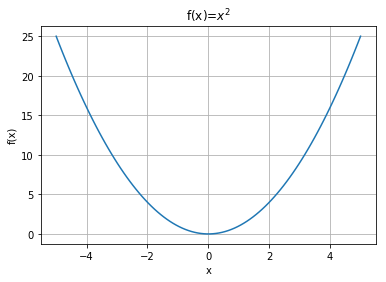
\includegraphics[width=0.6\linewidth]{files/xsquared-bf8f4ef5428ad1a3df92f0692e26abcd.png}
\caption[]{$f(x)=x^2$ plotted between $x= -5$ and $=+5$.}
\label{fig:calculus:xsquared}
\end{figure}

Plotting a function of 2 variables is a little trickier, since we need to do it in three dimensions (one axis for $x$, one axis for $y$, and one axis for $g(x,y)$). Figure~\ref{fig:calculus:gxy} shows an example of plotting a function of 2 variables.

\begin{figure}[!htbp]
\centering
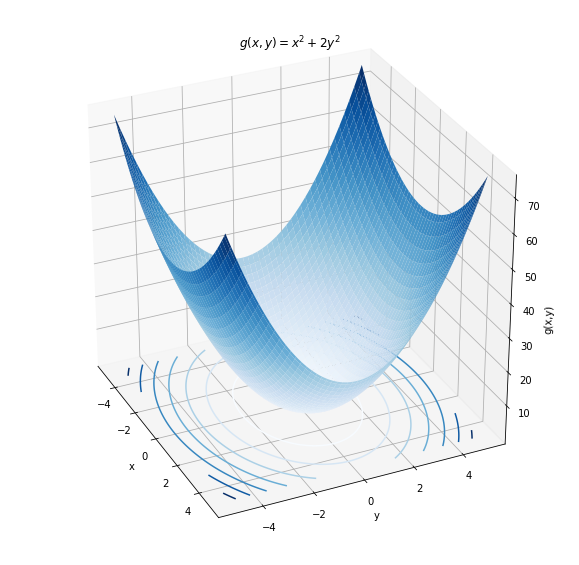
\includegraphics[width=0.6\linewidth]{files/gxy-16fd31f6194c2b2b9daab98c06eefc56.png}
\caption[]{$g(x,y)=x^2+2y^2$ plotted for $x$ between -5 and +5 and for $y$ between -5 and +5. A function of two variables can be visualized as a surface in three dimensions. One can also visualize the function by look at its ``contours'' (the lines drawn in the $xy$ plane).}
\label{fig:calculus:gxy}
\end{figure}

Unfortunately, it becomes difficult to visualize functions of more than 2 variables, although one can usually look at projections of those functions to try and visualize some of the features (for example, contour maps are 2D projections of 3D surfaces, as shown in the xy plane of Figure~\ref{fig:calculus:gxy}). When you encounter a function, it is good practice to try and visualize it if you can. For example, ask yourself the following questions:

\begin{itemize}
\item Does the function have one or more maxima and/or minima?
\item Does the function cross zero?
\item Is the function continuous everywhere?
\item Is the function always defined for any value of the independent variables?
\end{itemize}

\subsubsection{Derivatives}

Consider the function $f(x)=x^2$ that is plotted in Figure~\ref{fig:calculus:xsquared}. For any value of $x$, we can define the slope of the function as the ``steepness of the curve''. For values of $x>0$ the function increases as $x$ increases, so we say that the slope is positive. For values of $x<0$, the function decreases as $x$ increases, so we say that the slope is negative. A synonym for the word slope is ``derivative'', which is the word that we prefer to use in calculus. The derivative of a function $f(x)$ is given the symbol $\frac{df}{dx}$ to indicate that we are referring to the slope of $f(x)$ when plotted as a function of $x$.

We need to specify which variable we are taking the derivative with respect to when the function has more than one variable but only one of them should be considered \textit{independent}. For example, the function $f(x)=ax^2+b$ will have different values if $a$ and $b$ are changed, so we have to be precise in specifying that we are taking the derivative with respect to $x$. The following notations are equivalent ways to say that we are taking the derivative of $f(x)$ with respect to $x$:
\begin{equation}
\frac{df}{dx}=\frac{d}{dx} f(x) = f'(x) = f'
\end{equation}
The notation with the prime ($f'(x),f'$) can be useful to indicate that the derivative itself is \textit{also} a function of $x$.

The slope (derivative) of a function tells us how rapidly the value of the function is changing when the independent variable is changing. For $f(x)=x^2$, as $x$ gets more and more positive, the function gets steeper and steeper; the derivative is thus increasing with $x$. The sign of the derivative tells us if the function is increasing or decreasing, whereas its absolute value tells how quickly the function is changing (how steep it is).

We can approximate the derivative by evaluating how much $f(x)$ changes when $x$ changes by a small amount, say, $\Delta x$. In the limit of $\Delta x\to 0$, we get the derivative. In fact, this is the formal definition of the derivative:
\begin{equation}
\label{eqn:Calculus:derdef}
\boxed{\frac{df}{dx}=\lim_{\Delta x\to 0}\frac{\Delta f}{\Delta x} =\lim_{\Delta x\to 0}\frac{f(x+\Delta x)-f(x)}{\Delta x} }
\end{equation}
where $\Delta f$ is the small change in $f(x)$ that corresponds to the small change, $\Delta x$, in $x$. This makes the notation for the derivative more clear, $dx$ is $\Delta x$ in the limit where $\Delta x\to0$, and $df$ is $\Delta f$, in the same limit of $\Delta x\to 0$.

As an example, let us determine the function $f'(x)$ that is the derivative of $f(x)=x^2$. We start by calculating $\Delta f$:
\begin{equation}
\Delta f &= f(x+\Delta x)-f(x)\\
&=(x+\Delta x)^2 - x^2\\
&=x^2+2x\Delta x+\Delta x^2 -x^2\\
&=2x\Delta x+\Delta x^2
\end{equation}
We now calculate $\frac{\Delta f}{\Delta x}$:
\begin{equation}
\frac{\Delta f}{\Delta x}&=\frac{2x\Delta x+\Delta x^2}{\Delta x}\\
&=2x+\Delta x
\end{equation}
and take the limit $\Delta x\to 0$:
\begin{equation}
\frac{df}{dx}&=\lim_{\Delta x\to 0 }\frac{\Delta f}{\Delta x}\\
&=\lim_{\Delta x\to 0 }(2x+\Delta x)\\
&=2x
\end{equation}
We have thus found that the function, $f'(x)=2x$, is the derivative of the function $f(x)=x^2$. This is illustrated in Figure~\ref{fig:Calculus:ffprime}. Note that:

\begin{itemize}
\item For $x>0$, $f'(x)$ is positive and increasing with increasing $x$, just as we described earlier (the function $f(x)$ is increasing and getting steeper).
\item For $x<0$, $f'(x)$ is negative and decreasing in magnitude as $x$ increases. Thus $f(x)$ decreases and gets less steep as $x$ increases.
\item At $x=0$, $f'(x)=0$ indicating that, at the origin, the function $f(x)$ is (momentarily) flat.
\end{itemize}

\begin{figure}[!htbp]
\centering
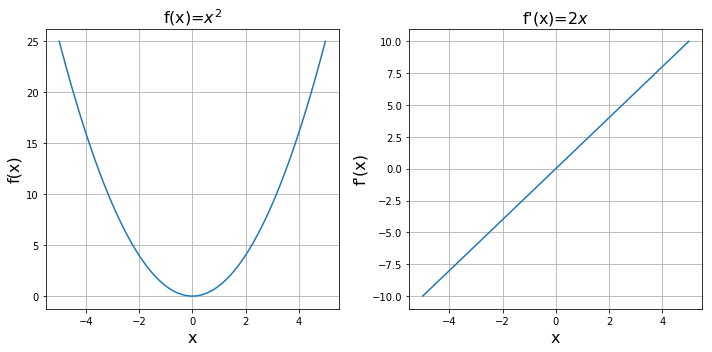
\includegraphics[width=0.9\linewidth]{files/ffprime-c8ca31b4706b09cd0bc7d2cab72c554a.png}
\caption[]{$f(x)=x^2$ and its derivative, $f'(x)=2x$ plotted for x between -5 and +5.}
\label{fig:Calculus:ffprime}
\end{figure}

\begin{framed}
\textbf{Checkpoint}\\
When a function has a maximum, its derivative at that point\}

\begin{enumerate}
\item also has a maximum
\item is zero
\item has a minimum
\item is infinite
\end{enumerate}

\begin{framed}
\textbf{Answer}\\
\begin{enumerate}[resume]
\item
\end{enumerate}
\end{framed}
\end{framed}

\paragraph{Common derivatives and properties}

It is beyond the scope of this document to derive the functional form of the derivative for any function using equation (\ref{eqn:Calculus:derdef}). Table~\ref{tab:Calculus:commonders} below gives the derivatives for common functions. In all cases, $x$ is the independent variable, and all other variables should be thought of as constants:

\begin{table}
\centering
\caption[]{Common derivatives of functions.}
\label{tab:Calculus:commonders}
\begin{tabular}{p{\dimexpr 0.500\linewidth-2\tabcolsep}p{\dimexpr 0.500\linewidth-2\tabcolsep}}
\toprule
\textbf{Function, $f(x)$} & \textbf{Derivative, $f'(x)$} \\
\hline
$f(x)=a$ & $f'(x)=0$ \\
$f(x)=x^n$ & $f'(x)=nx^{n -1}$ \\
$f(x)=\sin(x)$ & $f'(x)=\cos(x)$ \\
$f(x)=\cos(x)$ & $f'(x)= -\sin(x)$ \\
$f(x)=\tan(x)$ & $f'(x)=\frac{1}{\cos^2(x)}$ \\
$f(x)=e^x$ & $f'(x)=e^x$ \\
$f(x)=\ln(x)$ & $f'(x)=\frac{1}{x}$ \\
\bottomrule
\end{tabular}
\end{table}

If two functions of 1 variable, $f(x)$ and $g(x)$, are combined into a third function, $h(x)$, then there are simple rules for finding the derivative, $h'(x)$, based on the derivatives $f'(x)$ and $g'(x)$. These are summarized in Table~\ref{tab:Calculus:combders} below.

\begin{table}
\centering
\caption[]{Derivatives of combined functions.}
\label{tab:Calculus:combders}
\begin{tabular}{p{\dimexpr 0.500\linewidth-2\tabcolsep}p{\dimexpr 0.500\linewidth-2\tabcolsep}}
\toprule
\textbf{Function, $h(x)$} & \textbf{Derivative, $h'(x)$} \\
\hline
$h(x)=f(x)+g(x)$ & $h'(x)=f'(x)+g'(x)$ \\
$h(x)=f(x) -g(x)$ & $h'(x)=f'(x) -g'(x)$ \\
$h(x)=f(x)g(x)$ & $h'(x)=f'(x)g(x)+f(x)g'(x)$ (The product rule) \\
$h(x)=\frac{f(x)}{g(x)}$ & $h'(x)=\frac{f'(x)g(x) -f(x)g'(x)}{g^2(x)}$ (The quotient rule) \\
$h(x)=f(g(x))$ & $h'(x)=f'(g(x))g'(x)$ (The Chain Rule) \\
\bottomrule
\end{tabular}
\end{table}

\begin{framed}
\textbf{Example}\\
Use the properties from Table~\ref{tab:Calculus:combders} to show that the derivative of $\tan(x)$ is $\frac{1}{\cos^2(x)}$.

\begin{framed}
\textbf{Solution}\\
Since $\tan(x)=\frac{\sin(x)}{\cos(x)}$, we can write:
\begin{equation}
h(x) &= \frac{f(x)}{g(x)} \\
f(x) &= \sin(x)\\
g(x) &= \cos(x)
\end{equation}
Using the fourth row in Table~\ref{tab:Calculus:combders}, and the common derivatives from Table~\ref{tab:Calculus:commonders}, we have:
\begin{equation}
f'(x) &= \cos(x) \\
g'(x) &= -\sin(x) \\
g^2(x) &= \cos^2(x) \\
h'(x) &=\frac{f'(x)g(x)-f(x)g'(x)}{g^2(x)}\\ 
&= \frac{\cos(x)\cos(x) - \sin(x) (-\sin(x))}{\cos^2(x)}\\
&=\frac{\cos^2(x)+\sin^2(x)}{\cos^2(x)}\\
&=\frac{1}{\cos^2(x)}
\end{equation}
as required.
\end{framed}
\end{framed}

\begin{framed}
\textbf{Example}\\
Use the properties from Table~\ref{tab:Calculus:combders} to calculate the derivative of $h(x)=\sin^2(x)$.

\begin{framed}
\textbf{Solution}\\
To calculate the derivative of $h(x)$, we need to use the Chain Rule. $h(x)$ is found by first taking $\sin(x)$ and then taking that result squared. We can thus identify:
\begin{equation}
h(x) &= \sin^2(x) = f(g(x))\\
f(x) &= x^2 \\
g(x) &= \sin(x)
\end{equation}
Using the common derivatives from Table~\ref{tab:Calculus:commonders}, we have:
\begin{equation}
f'(x) &= 2x \\
g'(x) &= \cos(x)
\end{equation}
Applying the Chain Rule, we have:
\begin{equation}
h'(x) &= f'(g(x))g'(x)\\
&= 2\sin(x)g'(x)\\
&= 2\sin(x)\cos(x)
\end{equation}
where $f'(g(x))$ means apply the derivative of $f(x)$ to the function $g(x)$. Since the derivative of $f(x)$ is $f'(x)=2x$, when we apply it to $g(x)$ instead of $2x$, we get $2g(x)=2\cos(x)$.
\end{framed}
\end{framed}

\paragraph{Partial derivatives and gradients}\label{sec:Calculus:gradients}

So far, we have only looked at the derivative of a function of a single independent variable and used it to quantify how much the function changes when the independent variable changes. We can proceed analogously for a function of multiple variables, $f(x,y)$, by quantifying how much the function changes along the direction associated with a particular variable. This is illustrated in Figure~\ref{fig:Calculus:fxy} for the function $f(x,y)=x^2 -2y^2$, which looks somewhat like a saddle.

\begin{figure}[!htbp]
\centering
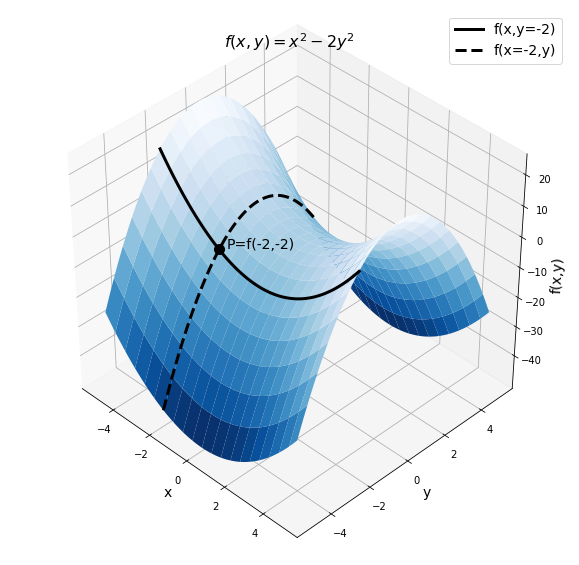
\includegraphics[width=0.7\linewidth]{files/fxy-5c7af468668da8d5d9149c8f84a65384.png}
\caption[]{$f(x,y)=x^2 -2y^2$ plotted for $x$ between -5 and +5 and for $y$ between -5 and +5. The point P labelled on the figure shows the value of the function at $f( -2, -2)$. The two lines show the function evaluated when one of $x$ or $y$ is held constant.}
\label{fig:Calculus:fxy}
\end{figure}

Suppose that we wish to determine the derivative of the function $f(x,y)$ at $x= -2$ and $y= -2$. In this case, it does not make sense to simply determine the ``derivative'', but rather, we must specify \textit{in which direction} we want the derivative. That is, we need to specify in which direction we are interested in quantifying the rate of change of the function.

One possibility is to quantify the rate of change in the $x$ direction. The solid line in Figure~\ref{fig:Calculus:fxy} shows the part of the function surface where $y$ is fixed at -2, that is, the function evaluated as $f(x,y= -2)$. The point $P$ on the figure shows the value of the function when $x= -2$ and $y= -2$. By looking at the solid line at point $P$, we can see that as $x$ increases, the value of the function is gently decreasing. The derivative of $f(x,y)$ with respect to $x$ when $y$ is held constant and evaluated at $x= -2$ and $y= -2$ is thus negative. Rather than saying ``The derivative of $f(x,y)$ with respect to $x$ when $y$ is held constant'' we say ``The \textbf{partial derivative} of $f(x,y)$ with respect to $x$''.

Since the partial derivative is different than the ordinary derivative (as it implies that we are holding independent variables fixed), we give it a different symbol, namely, we use $\partial$ instead of $d$:
\begin{equation}
\frac{\partial f}{\partial x}=\frac{\partial}{\partial x}f(x,y)\text{ (Partial derivative of f with respect to x)}
\end{equation}
Calculating the partial derivative is very easy, as we just treat all variables as constants except for the variable with respect to which we are differentiating\footnote{To take the derivative is to ``differentiate''!}. For the function $f(x,y)=x^2 -2y^2$, we have:
\begin{equation}
\frac{\partial f}{\partial x}&=\frac{\partial}{\partial x}\left(x^2-2y^2\right) = 2x\\
\frac{\partial f}{\partial y}&=\frac{\partial}{\partial y}\left(x^2-2y^2\right) = -4y
\end{equation}
At $x= -2$, the partial derivative of $f(x,y)$ is indeed negative, consistent with our observation that, along the solid line, at point $P$, the function is decreasing.

A function will have as many partial derivatives as it has independent variables. Also note that, just like a normal derivative, a partial derivative is still a function. The partial derivative with respect to a variable tells us how steep the function is in the direction in which that variable increases and whether it is increasing or decreasing.

\begin{framed}
\textbf{Example}\\
Determine the partial derivatives of $f(x,y,z)=ax^2+byz -\sin(z)$.

\begin{framed}
\textbf{Solution}\\
In this case, we have three partial derivatives to evaluate. Note that $a$ are $b$ constants and can be thought of as numbers that we do not know.
\begin{equation}
\frac{\partial f}{\partial x}&=\frac{\partial}{\partial x}\left(ax^2+byz-\sin(z)\right) = 2ax\\
\frac{\partial f}{\partial y}&=\frac{\partial}{\partial y}\left(ax^2+byz-\sin(z)\right) = bz \\
\frac{\partial f}{\partial z}&=\frac{\partial}{\partial z}\left(ax^2+byz-\sin(z)\right) = by-\cos(z)
\end{equation}
\end{framed}
\end{framed}

Since the partial derivatives tell us how the function changes in a particular direction, we can use them to find the direction in which the function changes \textit{the most rapidly}. For example, suppose that the surface from Figure~\ref{fig:Calculus:fxy} corresponds to a real physical surface and that we place a ball at point $P$. We wish to know in which direction the ball will roll. The direction that it will roll in is the opposite of the direction where $f(x,y)$ increases the most rapidly (i.e. it will roll in the direction where $f(x,y)$ decreases the most rapidly). The direction in which the function increases the most rapidly is called the ``gradient'' and denoted by $\nabla f(x,y)$.

Since the gradient is a direction, it cannot be represented by a single number. Rather, we use a ``vector'' to indicate this direction. Since $f(x,y)$ has two independent variables, the gradient will be a vector with two components. The components of the gradient are given by the partial derivatives:
\begin{equation}
\nabla f(x,y) = \frac{\partial f}{\partial x}\hat x+\frac{\partial f}{\partial y} \hat y
\end{equation}
where $\hat x$ and $\hat y$ are the unit vectors in the $x$ and $y$ directions, respectively (sometimes, the unit vectors are denoted $\hat i$ and $\hat j$). The direction of the gradient tells us in which direction the function increases the fastest, and the magnitude of the gradient tells us how much the function increases in that direction.

\begin{framed}
\textbf{Example}\\
Determine the gradient of the function $f(x,y)=x^2 -2y^2$ at the point $x= -2$ and $y= -2$.

\begin{framed}
\textbf{Solution}\\
We have already found the partial derivatives that we need to evaluate at $x= -2$ and $y= -2$:
\begin{equation}
\frac{\partial f}{\partial x}&= 2x\\
\frac{\partial f}{\partial y}&= -4y \\
\therefore \nabla f(x,y) &= \frac{\partial f}{\partial x}\hat x+\frac{\partial f}{\partial y} \hat y \\
&=2x\hat x-4y\hat y
\end{equation}
Evaluating the gradient at $x= -2$ and $y= -2$:
\begin{equation}
\nabla f(x,y) &= 2x\hat x-4y\hat y\\
&=-4 \hat x + 8 \hat y\\
&=4 (-\hat x+2\hat y)\\
\end{equation}
The gradient vector points in the direction $( -1,2)$. That is, the function increases the most in the direction where you would take 1 pace in the negative $x$ direction and 2 paces in the positive $y$ direction. You can confirm this by looking at point $P$ in Figure~\ref{fig:Calculus:fxy} and imagining in which direction you would have to go to climb the surface to get the steepest climb.
\end{framed}
\end{framed}

The gradient is itself a function, but it is not a real function (in the sense of a real number), since it evaluates to a vector. It is a mapping from real numbers $x,y$ to a vector. As you take more advanced calculus courses, you will eventually encounter ``vector calculus'', which is just the calculus for functions of multiple variables to which you were just introduced. The key point to remember here is that the gradient can be used to find the vector that points in the direction of maximal increase of the corresponding multi-variate function. This is precisely the quantity that we need in physics to determine in which direction a ball will roll when placed on a surface (it will roll in the direction opposite to the gradient vector).

\begin{framed}
\textbf{Checkpoint}\\
The gradient of a function of one variable, $f(x)$, is

\begin{enumerate}
\item undefined
\item zero
\item equal to its derivative
\item infinite
\end{enumerate}

\begin{framed}
\textbf{Answer}\\
\begin{enumerate}[resume]
\item
\end{enumerate}
\end{framed}
\end{framed}

\paragraph{Common uses of derivatives in physics}

The simplest case of using a derivative is to describe the speed of an object. If an object covers a distance $\Delta x$ in a period of time $\Delta t$, it's ``average speed'', $v_{avg}$, is defined as the distance covered by the object divided by the amount of time it took to cover that distance:
\begin{equation}
v_{avg} = \frac{\Delta x}{\Delta t}
\end{equation}
If the object changes speed (for example it is slowing down) over the distance $\Delta x$, we can still define its ``instantaneous speed'', $v$, by measuring the amount of time, $\Delta t$, that it takes the object to cover a \textit{very small distance}, $\Delta x$. The instantaneous speed is defined in the limit where $\Delta x \to 0$:
\begin{equation}
v = \lim_{\Delta x\to 0}\frac{\Delta x}{\Delta t}=\frac{dx}{dt}
\end{equation}
which is precisely the derivative of $x(t)$ with respect to $t$. $x(t)$ is a function that gives the position, $x$, of the object along some $x$ axis as a function of time. The speed of the object is thus the rate of change of its position.

Similarly, if the speed is changing with time, then we can define the ``acceleration'', $a$, of an object as the rate of change of its speed:
\begin{equation}
a = \frac{dv}{dt}
\end{equation}

\subsubsection{Anti-derivatives and integrals}\label{sec:calculus:integrals}

In the previous section, we were concerned with determining the derivative of a function $f(x)$. The derivative is useful because it tells us how the function $f(x)$ varies as a function of $x$. In physics, we often know how a function varies, but we do not know the actual function. In other words, we often have the opposite problem: we are given the derivative of a function, and wish to determine the actual function. For this case, we will limit our discussion to functions of a single independent variable.

Suppose that we are given a function $f(x)$ and we know that this is the derivative of some other function, $F(x)$, which we do not know. We call $F(x)$ the \textbf{anti-derivative} of $f(x)$. The anti-derivative of a function $f(x)$, written $F(x)$, thus satisfies the property:
\begin{equation}
\frac{dF}{dx}=f(x)
\end{equation}
Since we have a symbol for indicating that we take the derivative with respect to $x$ ($\frac{d}{dx}$), we also have a symbol, $\int dx$, for indicating that we take the anti-derivative with respect to $x$:
\begin{equation}
\int f(x) dx &= F(x) \\
\therefore \frac{d}{dx}\left(\int f(x) dx\right) &= \frac{dF}{dx}=f(x)
\end{equation}
Earlier, we justified the symbol for the derivative by pointing out that it is like $\frac{\Delta f}{\Delta x}$ but for the case when $\Delta x\to 0$. Similarly, we will justify the anti-derivative sign, $\int f(x) dx$, by showing that it is related to a sum of $f(x)\Delta x$, in the limit $\Delta x\to 0$. The $\int$ sign looks like an ``S'' for sum.

While it is possible to exactly determine the derivative of a function $f(x)$, the anti-derivative can only be determined up to a constant. Consider for example a different function, $\tilde F(x)=F(x)+C$, where $C$ is a constant. The derivative of $\tilde F(x)$ with respect to $x$ is given by:
\begin{equation}
\frac{d\tilde{F}}{dx}&=\frac{d}{dx}\left(F(x)+C\right)\\
&=\frac{dF}{dx}+\frac{dC}{dx}\\
&=\frac{dF}{dx}+0\\
&=f(x)
\end{equation}
Hence, the function $\tilde F(x)=F(x)+C$ is also an anti-derivative of $f(x)$. The constant $C$ can often be determined using additional information (sometimes called ``initial conditions''). Recall the function, $f(x)=x^2$, shown in Figure~\ref{fig:Calculus:ffprime} (left panel). If you imagine shifting the whole function up or down, the derivative would not change. In other words, if the origin of the axes were not drawn on the left panel, you would still be able to determine the derivative of the function (how steep it is). Adding a constant, $C$, to a function is exactly the same as shifting the function up or down, which does not change its derivative. Thus, when you know the derivative, you cannot know the value of $C$, unless you are also told that the function must go through a specific point (a so-called initial condition).

In order to determine the derivative of a function, we used equation (\ref{eqn:Calculus:derdef}). We now need to derive an equivalent prescription for determining the anti-derivative. Suppose that we have the two pieces of information required to determine $F(x)$ completely, namely:

\begin{enumerate}
\item the function $f(x)=\frac{dF}{dx}$ (its derivative).
\item the condition that $F(x)$ must pass through a specific point, $F(x_0)=F_0$.
\end{enumerate}

\begin{figure}[!htbp]
\centering
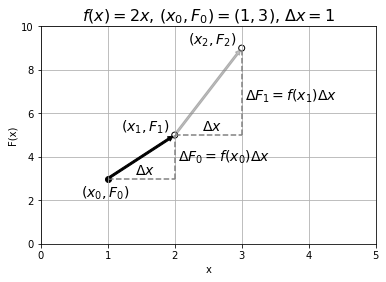
\includegraphics[width=0.6\linewidth]{files/fint-9d8441552867bce7c1dce2d0c105defd.png}
\caption[]{Determining the anti-derivative, $F(x)$, given the function $f(x)=2x$ and the initial condition that $F(x)$ passes through the point $(x_0,F_0)=(1,3)$.}
\label{fig:Calculus:fint}
\end{figure}

The procedure for determining the anti-derivative $F(x)$ is illustrated above in Figure~\ref{fig:Calculus:fint}. We start by drawing the point that we know the function $F(x)$ must go through, $(x_0,F_0)$. We then choose a value of $\Delta x$ and use the derivative, $f(x)$, to calculate $\Delta F_0$, the amount by which $F(x)$ changes when $x$ changes by $\Delta x$. Using the derivative $f(x)$ evaluated at $x_0$, we have:
\begin{equation}
\frac{\Delta F_0}{\Delta x} &\approx f(x_0)\;\;\;\; (\text{in the limit} \Delta x\to 0 )\\
\therefore \Delta F_0 &= f(x_0) \Delta x
\end{equation}
We can then estimate the value of the function $F_1=F(x_1)$ at the next point, $x_1=x_0+\Delta x$, as illustrated by the black arrow in Figure~\ref{fig:Calculus:fint}
\begin{equation}
F_1&=F(x_1)\\
&=F(x+\Delta x) \\
&\approx F_0 + \Delta F_0\\
&\approx F_0+f(x_0)\Delta x
\end{equation}
Now that we have determined the value of the function $F(x)$ at $x=x_1$, we can repeat the procedure to determine the value of the function $F(x)$ at the next point, $x_2=x_1+\Delta x$. Again, we use the derivative evaluated at $x_1$, $f(x_1)$, to determine $\Delta F_1$, and add that to $F_1$ to get $F_2=F(x_2)$, as illustrated by the grey arrow in Figure~\ref{fig:Calculus:fint}:
\begin{equation}
F_2&=F(x_1+\Delta x) \\
&\approx F_1+\Delta F_1\\
&\approx F_1+f(x_1)\Delta x\\
&\approx F_0+f(x_0)\Delta x+f(x_1)\Delta x
\end{equation}
Using the summation notation, we can generalize the result and write the function $F(x)$ evaluated at any point, $x_N=x_0+N\Delta x$:
\begin{equation}
F(x_N) \approx F_0+\sum_{i=1}^{i=N} f(x_{i-1}) \Delta x
\end{equation}
The result above will become exactly correct in the limit $\Delta x\to 0$:
\begin{equation}
\label{eqn:Calculus:intsum}
F(x_N) = F(x_0)+\lim_{\Delta x\to 0}\sum_{i=1}^{i=N} f(x_{i-1}) \Delta x
\end{equation}
Let us take a closer look at the sum. Each term in the sum is of the form $f(x_{i -1})\Delta x$, and is illustrated in Figure~\ref{fig:Calculus:fintarea} for the same case as in Figure~\ref{fig:Calculus:fint} (that is, Figure~\ref{fig:Calculus:fintarea} shows $f(x)$ that we know, and Figure~\ref{fig:Calculus:fint} shows $F(x)$ that we are trying to find).

\begin{figure}[!htbp]
\centering
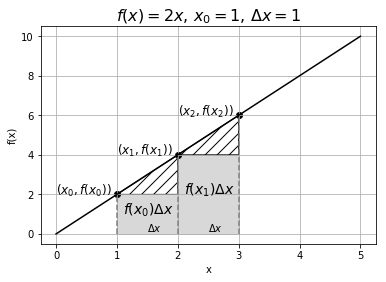
\includegraphics[width=0.6\linewidth]{files/fintarea-0c92a33946251b1a236108957256cebd.png}
\caption[]{The function $f(x)=2x$ and illustration of the terms $f(x_0)\Delta x$ and $f(x_1)\Delta x$ as the area between the curve $f(x)$ and the $x$ axis when $\Delta x\to 0$.}
\label{fig:Calculus:fintarea}
\end{figure}

As you can see, each term in the sum corresponds to the area of a rectangle between the function $f(x)$ and the $x$ axis (with a piece missing). In the limit where $\Delta x\to 0$, the missing pieces (shown by the hashed areas in Figure~\ref{fig:Calculus:fintarea}) will vanish and $f(x_i)\Delta x$ will become exactly the area between $f(x)$ and the $x$ axis over a length $\Delta x$. The sum of the rectangular areas will thus approach the area between $f(x)$ and the  $x$ axis between $x_0$ and $x_N$:
\begin{equation}
\lim_{\Delta x\to 0}\sum_{i=1}^{i=N} f(x_{i-1}) \Delta x=\text{Area between f(x) and x axis from $x_0$ to $x_N$}
\end{equation}

Re-arranging equation (\ref{eqn:Calculus:intsum}) gives us a prescription for determining the anti-derivative:
\begin{equation}
F(x_N) - F(x_0)&=\lim_{\Delta x\to 0}\sum_{i=1}^{i=N} f(x_{i-1}) \Delta x
\end{equation}
We see that if we determine the area between $f(x)$ and the $x$ axis from $x_0$ to $x_N$, we can obtain the difference between the anti-derivative at two points, $F(x_N) -F(x_0)$

The difference between the anti-derivative, $F(x)$, evaluated at two different values of $x$ is called the \textbf{integral} of $f(x)$ and has the following notation:
\begin{equation}
\label{eqn:Calculus:intdef}
\boxed{\int_{x_0}^{x_N}f(x) dx=F(x_N) - F(x_0)=\lim_{\Delta x\to 0}\sum_{i=1}^{i=N} f(x_{i-1}) \Delta x}
\end{equation}
As you can see, the integral has labels that specify the range over which we calculate the area between $f(x)$ and the $x$ axis. A common notation to express the difference $F(x_N) - F(x_0)$ is to use brackets:
\begin{equation}
\int_{x_0}^{x_N}f(x) dx=F(x_N) - F(x_0) =\big [ F(x) \big]_{x_0}^{x_N}
\end{equation}

Recall that we wrote the anti-derivative with the same $\int$ symbol earlier:
\begin{equation}
\int f(x) dx = F(x)
\end{equation}
The symbol $\int f(x) dx$ without the limits is called the \textbf{indefinite integral}. You can also see that when you take the (definite) integral (i.e. the  difference between $F(x)$ evaluated at two points), any constant that is added to $F(x)$ will cancel. Physical quantities are always based on definite integrals, so when we write the constant $C$ it is primarily for completeness and to emphasize that we have an indefinite integral.

As an example, let us determine the integral of $f(x)=2x$ between $x=1$ and $x=4$, as well as the indefinite integral of $f(x)$, which is the case that we illustrated in Figures {\textbackslash}ref\{fig:Calculus:fint\} and {\textbackslash}ref\{fig:Calculus:fintarea\}. Using equation (\ref{eqn:Calculus:intdef}), we have:
\begin{equation}
\int_{x_0}^{x_N}f(x) dx&=\lim_{\Delta x\to 0}\sum_{i=1}^{i=N} f(x_{i-1}) \Delta x \\
&=\lim_{\Delta x\to 0}\sum_{i=1}^{i=N} 2x_{i-1} \Delta x
\end{equation}
where we have:
\begin{equation}
x_0 &=1 \\
x_N &=4 \\
\Delta x &= \frac{x_N-x_0}{N}
\end{equation}
Note that $N$ is the number of times we have $\Delta x$ in the interval between $x_0$ and $x_N$. Thus, taking the limit of $\Delta x\to 0$ is the same as taking the limit $N\to\infty$. Let us illustrate the sum for the case where $N=3$, and thus when $\Delta x=1$, corresponding to the illustration in Figure~\ref{fig:Calculus:fintarea}:
\begin{equation}
\sum_{i=1}^{i=N=3} 2x_{i-1} \Delta x &=2x_0\Delta x+2x_1\Delta x+2x_2\Delta x\\
&=2\Delta x (x_0+x_1+x_2) \\
&=2 \frac{x_3-x_0}{N}(x_0+x_1+x_2) \\
&=2 \frac{(4)-(1)}{(3)}(1+2+3) \\
&=12
\end{equation}
where in the second line, we noticed that we could factor out the $2\Delta x$ because it appears in each term. Since we only used 4 points, this is a pretty coarse approximation of the integral, and we expect it to be an underestimate (as the missing area represented by the hashed lines in Figure~\ref{fig:Calculus:fintarea} is quite large).

If we repeat this for a larger value of N, $N=6$ ($\Delta x = 0.5$), we should obtain a more accurate answer:
\begin{equation}
\sum_{i=1}^{i=6} 2x_{i-1} \Delta x &=2 \frac{x_6-x_0}{N}(x_0+x_1+x_2+x_3+x_4+x_5)\\
&=2\frac{4-1}{6} (1+1.5+2+2.5+3+3.5)\\
&=13.5
\end{equation}

Writing this out again for the general case so that we can take the limit $N\to\infty$, and factoring out the $2\Delta x$:
\begin{equation}
\sum_{i=1}^{i=N} 2x_{i-1} \Delta x &=2 \Delta x\sum_{i=1}^{i=N}x_{i-1}\\
&=2 \frac{x_N-x_0}{N}\sum_{i=1}^{i=N}x_{i-1}
\end{equation}
Now, consider the combination:
\begin{equation}
\frac{1}{N}\sum_{i=1}^{i=N}x_{i-1}
\end{equation}
that appears above. This corresponds to the arithmetic average of the values from $x_0$ to $x_{N -1}$ (sum the values and divide by the number of values). In the limit where $N\to \infty$, then the value $x_{N -1}\approx x_N$. The average value of $x$ in the interval between $x_0$ and $x_N$ is simply given by the value of $x$ at the midpoint of the interval:
\begin{equation}
\lim_{N\to\infty}\frac{1}{N}\sum_{i=1}^{i=N}x_{i-1}=\frac{1}{2}(x_N+x_0)
\end{equation}
Putting everything together:
\begin{equation}
\lim_{N\to\infty}\sum_{i=1}^{i=N} 2x_{i-1} \Delta x &=2 (x_N+x_0)\lim_{N\to\infty}\frac{1}{N}\sum_{i=1}^{i=N}x_{i-1}\\
&=2 (x_N-x_0)\frac{1}{2}(x_N+x_0)\\
&=x_N^2 - x_0^2\\
&=(4)^2 - (1)^2 = 15
\end{equation}
where in the last line, we substituted in the values of $x_0=1$ and $x_N=4$. Writing this as the integral:
\begin{equation}
\int_{x_0}^{x_N}2x dx=F(x_N) - F(x_0)=x_N^2 - x_0^2
\end{equation}
we can immediately identify the anti-derivative and the indefinite integral:
\begin{equation}
F(x) &= x^2 +C \\
\int 2xdx&=x^2 +C
\end{equation}
This is of course the result that we expected, and we can check our answer by taking the derivative of $F(x)$:
\begin{equation}
\frac{dF}{dx}=\frac{d}{dx}(x^2+C) = 2x
\end{equation}
We have thus confirmed that $F(x)=x^2+C$ is the anti-derivative of $f(x)=2x$.

\begin{framed}
\textbf{Checkpoint}\\
The quantity $\int_{a}^{b}f(t)dt$ is equal to

\begin{enumerate}
\item the area between the function $f(t)$ and the $f$ axis between $t=a$ and $t=b$
\item the sum of $f(t)\Delta t$ in the limit $\Delta t\to 0$ between $t=a$ and $t=b$
\item the difference $f(b) - f(a)$.
\end{enumerate}

\begin{framed}
\textbf{Answer}\\
\begin{enumerate}[resume]
\item
\end{enumerate}
\end{framed}
\end{framed}

\paragraph{Common anti-derivative and properties}

Table~\ref{tab:Calculus:commonints} below gives the anti-derivatives (indefinite integrals) for common functions. In all cases, $x,$ is the independent variable, and all other variables should be thought of as constants:

\begin{table}
\centering
\caption[]{Common indefinite integrals of functions.}
\label{tab:Calculus:commonints}
\begin{tabular}{p{\dimexpr 0.500\linewidth-2\tabcolsep}p{\dimexpr 0.500\linewidth-2\tabcolsep}}
\toprule
\textbf{Function, $f(x)$} & \textbf{Anti-derivative, $F(x)$} \\
\hline
$f(x)=a$ & $F(x)=ax+C$ \\
$f(x)=x^n$ & $F(x)=\frac{1}{n+1}x^{n+1}+C$ \\
$f(x)=\frac{1}{x}$ & \$F(x)={\textbackslash}ln( \\
$f(x)=\sin(x)$ & $F(x)= -\cos(x)+C$ \\
$f(x)=\cos(x)$ & $F(x)=\sin(x)+C$ \\
$f(x)=\tan(x)$ & $F(x)= -\ln\left(\left|\cos(x)\right|\right)+C$ \\
$f(x)=e^x$ & $F(x)=e^x+C$ \\
$f(x)=\ln(x)$ & $F(x)=x\ln(x) -x+C$ \\
\bottomrule
\end{tabular}
\end{table}

Note that, in general, it is much more difficult to obtain the anti-derivative of a function than it is to take its derivative. A few common properties to help evaluate indefinite integrals are shown in Table~\ref{tab:Calculus:intprops} below.

\begin{table}
\centering
\caption[]{Some properties of indefinite integrals.}
\label{tab:Calculus:intprops}
\begin{tabular}{p{\dimexpr 0.500\linewidth-2\tabcolsep}p{\dimexpr 0.500\linewidth-2\tabcolsep}}
\toprule
\textbf{Anti-derivative} & \textbf{Equivalent anti-derivative} \\
\hline
$\int (f(x)+g(x)) dx$ & $\int f(x)dx+\int g(x) dx$ (sum) \\
$\int (f(x) -g(x)) dx$ & $\int f(x)dx -\int g(x) dx$ (subtraction) \\
$\int af(x) dx$ & $a\int f(x)dx$ (multiplication by constant) \\
$\int f'(x)g(x) dx$ & $f(x)g(x) -\int f(x)g'(x) dx$ (integration by parts) \\
\bottomrule
\end{tabular}
\end{table}

\paragraph{Common uses of integrals in Physics - from a sum to an integral}

Integrals are extremely useful in physics because they are related to sums. If we assume that our mathematician friends (or computers) can determine anti-derivatives for us, using integrals is not that complicated.

The key idea in physics is that \textbf{integrals are a tool to easily performing sums}. As we saw above, integrals correspond to the area underneath a curve, which is found by \textit{summing} the (different) areas of an infinite number of infinitely small rectangles. In physics, it is often the case that we need to take the sum of an infinite number of small things that keep varying, just as the areas of the rectangles.

Consider, for example, a rod of length, $L$, and total mass $M$, as shown in Figure~\ref{fig:Calculus:rod}. If the rod is uniform in density, then if we cut it into, say, two equal pieces, those two pieces will weigh the same. We can define a ``linear mass density'', $\mu$, for the rod, as the mass per unit length of the rod:
\begin{equation}
\mu = \frac{M}{L}
\end{equation}
The linear mass density has dimensions of mass over length and can be used to find the mass of any length of rod. For example, if the rod has a mass of $M=5 {\rm kg}$ and a length of $L=2 {\rm m}$, then the mass density is:
\begin{equation}
\mu=\frac{M}{L}=\frac{(5 {\rm kg})}{(2 {\rm m})}=2.5 {\rm kg/m}
\end{equation}
Knowing the mass density, we can now easily find the mass, $m$, of a piece of rod that has a length of, say, $l=10 {\rm cm}$. Using the mass density, the mass of the $10 {\rm cm}$ rod is given by:
\begin{equation}
m=\mu l=(2.5 {\rm kg/m})(0.1 {\rm m})=0.25 {\rm kg}
\end{equation}
Now suppose that we have a rod of length $L$ that is not uniform, as in Figure~\ref{fig:Calculus:rod}, and that does not have a constant linear mass density. Perhaps the rod gets wider and wider, or it has holes in it that make it not uniform. Imagine that the mass density of the rod is instead given by a function, $\mu(x)$, that depends on the position along the rod, where $x$ is the distance measured from one side of the rod.

\begin{figure}[!htbp]
\centering
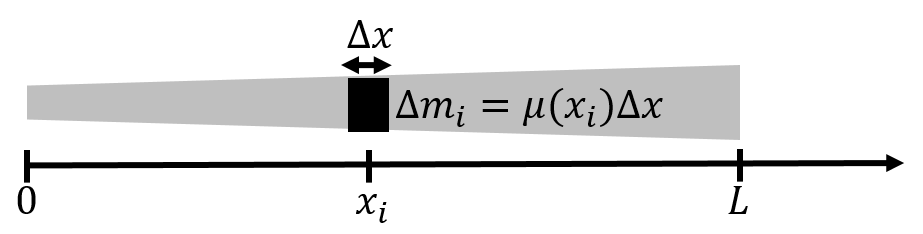
\includegraphics[width=0.7\linewidth]{files/rod-59833f0247eca084126948bbbd21f631.png}
\caption[]{A rod with a varying linear density. To calculate the mass of the rod, we consider a small mass element $\Delta m_i$ of length $\Delta x$ at position $x_i$. The total mass of the rod is found by summing the mass of the small mass elements.}
\label{fig:Calculus:rod}
\end{figure}

Now, we cannot simply determine the mass of the rod by multiplying $\mu(x)$ and $L$, since we do not know which value of $x$ to use. In fact, we have to use all of the values of $x$, between $x=0$ and $x=L$.

The strategy is to divide the rod up into $N$ pieces of length $\Delta x$. If we label our pieces of rod with an index $i$, we can say that the piece that is at position $x_i$ has a tiny mass, $\Delta m_i$. We assume that $\Delta x$ is small enough so that $\mu(x)$ can be taken as constant over the length of that tiny piece of rod. Then, the tiny piece of rod at $x=x_i$, has a mass, $\Delta m_i$, given by:
\begin{equation}
\Delta m_i = \mu(x_i) \Delta x
\end{equation}
where $\mu(x_i)$ is evaluated at the position, $x_i$, of our tiny piece of rod. The total mass, $M$, of the rod is then the sum of the masses of the tiny rods, in the limit where $\Delta x\to 0$:
\begin{equation}
M &= \lim_{\Delta x\to 0}\sum_{i=1}^{i=N}\Delta m_i \\
  &= \lim_{\Delta x\to 0}\sum_{i=1}^{i=N} \mu(x_i) \Delta x
\end{equation}
But this is precisely the definition of the integral (equation (\ref{eqn:Calculus:intsum})), which we can easily evaluate with an anti-derivative:
\begin{equation}
M &=\lim_{\Delta x\to 0}\sum_{i=1}^{i=N} \mu(x_i) \Delta x \\
  &= \int_0^L \mu(x) dx \\
  &= G(L) - G(0)
\end{equation}
where $G(x)$ is the anti-derivative of $\mu(x)$.

Suppose that the mass density is given by the function:
\begin{equation}
\mu(x)=ax^3
\end{equation}
with anti-derivative (Table {\textbackslash}ref\{tab:Calculus:commonints\}):
\begin{equation}
G(x)=a\frac{1}{4}x^4 + C
\end{equation}
Let $a=5 {\rm kg/m^4}$ and let's say that the length of the rod is $L=0.5 {\rm m}$. The total mass of the rod is then:
\begin{equation}
M&=\int_0^L \mu(x) dx \\
&=\int_0^L ax^3 dx \\
&= G(L)-G(0)\\
&=\left[ a\frac{1}{4}L^4 \right] - \left[ a\frac{1}{4}0^4 \right]\\
&=5 {\rm kg/m^4}\frac{1}{4}(0.5 {\rm m})^4 \\
&=78 {\rm g}\\
\end{equation}

With a little practice, you can solve this type of problem without writing out the sum explicitly. Picture an \textit{infinitesimal} piece of the rod of length $dx$ at position $x$. It will have an \textit{infinitesimal} mass, $dm$, given by:
\begin{equation}
dm = \mu(x) dx
\end{equation}
The total mass of the rod is the then the sum (i.e. the integral) of the mass \textit{elements}
\begin{equation}
M = \int dm
\end{equation}
and we really can think of the $\int$ sign as a sum, when the things being summed are \textit{infinitesimally} small. In the above equation, we still have not specified the range in $x$ over which we want to take the sum; that is, we need some sort of index for the mass elements to make this a meaningful definite integral. Since we already know how to express $dm$ in terms of $dx$, we can substitute our expression for $dm$ using one with $dx$:
\begin{equation}
M = \int dm = \int_0^L \mu(x) dx
\end{equation}
where we have made the integral definite by specifying the range over which to sum, since we can use $x$ to ``label'' the mass elements.

One should note that coming up with the above integral is physics. Solving it is math. We will worry much more about writing out the integral than evaluating its value. Evaluating the integral can always be done by a mathematician friend or a computer, but determining which integral to write down is the physicist's job!

\subsubsection{Summary}

The derivative of a function, $f(x)$, with respect to $x$ can be written as:
\begin{equation}
\frac{d}{dx} f(x)=\frac{df}{dx}=f'(x)
\end{equation}
and measures the rate of change of the function with respect to $x$. The derivative of a function is generally itself a function. The derivative is defined as:
\begin{equation}
f'(x) = \lim_{\Delta x \to 0}\frac{f(x+\Delta x)-f(x)}{\Delta x}
\end{equation}
Graphically, the derivative of a function represents the slope of the function, and it is positive if the function is increasing, negative if the function is decreasing and zero if the function is flat.  Derivatives can always be determined analytically for any continuous function.

A partial derivative measures the rate of change of a multi-variate function, $f(x,y)$, with respect to one of its independent variables. The partial derivative with respect to one of the variables is evaluated by taking the derivative of the function with respect to that variable while treating all other independent variables as if they were constant. The partial derivative of a function (with respect to $x$) is written as:
\begin{equation}
\frac{\partial f}{\partial x}
\end{equation}
The gradient of a function, $\nabla f(x,y)$, is a vector in the direction in which that function is increasing most rapidly. It is given by:
\begin{equation}
\nabla f(x,y)=\frac{\partial f}{\partial x}\hat x + \frac{\partial f}{\partial y} \hat y
\end{equation}

Given a function, $f(x)$, its anti-derivative with respect to $x$, $F(x)$, is written:
\begin{equation}
F(x) = \int f(x) dx
\end{equation}
$F(x)$ is such that its derivative with respect to $x$ is $f(x)$:
\begin{equation}
\frac{dF}{dx}=f(x)
\end{equation}
The anti-derivative of a function is only ever defined up to a constant, $C$. We usually write this as:
\begin{equation}
\int f(x) dx = F(x) + C
\end{equation}
since the derivative of $F(x) +C$ will also be equal to $f(x)$. The anti-derivative is also called the ``indefinite integral'' of $f(x)$.

The definite integral of a function $f(x)$, between $x=a$ and $x=b$, is written:
\begin{equation}
\int_a^b f(x) dx
\end{equation}
and is equal to the difference in the anti-derivative evaluated at $x=a$ and $x=b$:
\begin{equation}
\int_a^b f(x) dx = F(b) - F(a)
\end{equation}
where the constant $C$ no longer matters, since it cancels out. Physical quantities only ever depend on definite integrals, since they must be determined without an arbitrary constant.

Definite integrals are very useful in physics because they are related to a sum. Given a function $f(x)$, one can relate the sum of terms of the form $f(x_i)\Delta x$ over a range of values from $x=a$ to $x=b$ to the integral of $f(x)$ over that range:
\begin{equation}
\lim_{\Delta x\to 0}\sum_{i=1}^{i=N} f(x_{i-1}) \Delta x = \int_{x_0}^{x_N}f(x) dx=F(x_N) - F(x_0)=
\end{equation}

\subsubsection{Thinking about the Material}

\begin{framed}
\textbf{Reflect and research}\\
\begin{itemize}
\item When was calculus first discovered, and by whom?
\item What is an example of a physical quantity that is given by a derivative (other than speed or acceleration)?
\item What is a case when you would need to perform an integral to evaluate a physical quantity?
\end{itemize}
\end{framed}

\subsubsection{Sample problems and solutions}

\paragraph{Problems}

\begin{framed}
\textbf{Problem A.1}\\
You find that the number of customers in your store as a function of time is given by:
\begin{equation}
N(t) = a+bt-ct^2
\end{equation}
where $a$, $b$ and $c$ are constants. At what time does your store have the most customers, and what will the number of customers be? (Give the answer in terms of $a$, $b$ and $c$).
\end{framed}

\begin{framed}
\textbf{Problem A.2}\\
You measure the speed, $v(t)$, of an accelerating train as function of time, $t$, to be given by:
\begin{equation}
v(t)=at+bt^2
\end{equation}
where $a$ and $b$ are constants. How far does the train move between $t=t_0$ and $t=t_1$?
\end{framed}

\paragraph{Solutions}

\begin{framed}
\textbf{Solution A.1}\\
We need to find the value of $t$ for which the function $N(t)$ is maximal. This will occur when its derivative with respect to $t$ is zero:
\begin{equation}
\frac{dN}{dt} &= b-2ct =0\\
\therefore t &= \frac{b}{2c}
\end{equation}
At that time, the number of customers will be:
\begin{equation}
N\left( t=\frac{b}{2c} \right) &=a+bt-ct^2\\
&=a+\frac{b^2}{2c} - \frac{b^2}{4c} = a+\frac{b^2}{4c}
\end{equation}
\end{framed}

\begin{framed}
\textbf{Solution A.2}\\
We are given the speed of the train as a function of time, which is the rate of change of its position:
\begin{equation}
v(t)=\frac{dx}{dt}
\end{equation}
We need to find how its position, $x(t)$, changes with time, given the speed. In other words, we need to find the anti-derivative of $v(t)$ to get the function for the position as a function of time, $x(t)$:
\begin{equation}
x(t) &= \int v(t) dt = \int (at+bt^2) dt\\
&=\frac{1}{2}at^2 + \frac{1}{3}bt^3 + C
\end{equation}
where $C$ is an arbitrary constant. The distance covered, $\Delta x$, between time $t_0$ and time $t_1$ is simply the difference in position at those two times:
\begin{equation}
\Delta x &= x(t_1) - x(t_0)\\
&=\frac{1}{2}at_1^2 + \frac{1}{3}bt_1^3 + C - \frac{1}{2}at_0^2 - \frac{1}{3}bt_0^3 - C\\
&=\frac{1}{2}a(t_1^2-t_0^2) + \frac{1}{3}b(t_1^3-t_0^3)
\end{equation}
\end{framed}